%-------------------------------------------------------------------------------
\section{Introduction}
%-------------------------------------------------------------------------------
Web applications today own, process, and store user data~\cite{nytimes:fb, npr:data}.  This places a
great responsibility on application developers to transparently convey to users how they manage this
data via their privacy policies and terms of use.
%
\ms{next sentence doesn't follow: privacy policies + ToS doesn't imply data masks.}
Recent developments have renewed efforts to improve the state of data management in web
applications, creating incentives to support different forms of \emph{data masks}.

For example, applications mask data to hide a users' identity, performing privacy-preserving user
unsubscription from a service as mandated by laws such as the EU's General Data Protection
Regulation (GDPR)~\cite{eu:gdpr} and California's Consumer Privacy Act (CCPA)~\cite{ca:privacy-act}
that codify users' rights to data ownership and right to be forgotten. Unsubscription motivates a
need for an identify-revealing resubscription transformation, making it easy for users to return
instead of forcing users to permanently give up their accounts.

Growing incentives to keep as little compromising data as possible in case of a data
breach~\cite{breach:amazon,breach:twitter, breach:fb, breach:marriott, breach:quora} prompt
applications to mask stale or inactive users' data via anonymization or deletion. Similarly,
applications want to mask data that is stored in backups, or given to others for data processing.

%Data masks also go beyond just masking user data: applications apply masks to moderate
%harmful data (\eg inappropriate content or misinformation) that hide or modify data
%contents~\cite{contentmod, sasb}, and face increasing pressure from users who want to
%hold them legally liable for appropriately moderating content~\cite{nytimes:230}.

Properly specifying and implementing these various data masks is challenging. Masks are necessarily
application-specific and require the developer to reason about and handle complex data correlations.
For example, developers must selectively retain unsubscribing users' data for legal or application
purposes, while de-identifying this data as much as possible and maintaining application semantics.
Today's applications often support only coarse-grained masks implemented with ad-hoc methods,
resulting in a lack of a clear specification of exactly what and how the mask transforms data.

To help developers of new and existing applications support clearly specified data masks, we propose
\sys, a framework that, given only a high-level, declarative specification of the relationships
between entities in a database, generates and applies complex transformations that would be
laborious to implement manually. We observe that applications already encode entity
relations in an \emph{entity graph} via foreign key relationships, and this graph provides a means
for \sys to systematically reason about and automate a variety of data masks.
%To help developers of new and existing applications support privatization transformations, we
%propose \sys, which makes the key insight to model application data as an abstract \emph{entity
%graph}, and represent privatization transformations as transformations of this graph that render
%particular entities private.

With \sys, developers specify a \emph{mask policy} by choosing from a menu of provided edge and node
transformations. To determine an appropriate policy, developers introduce \emph{ghost entities} in the entity graph, which allow the mask to both retain, decorrelate, modify,
and remove data. The policy acts as a specification for the masked state of any instance of the
entity graph. When invoked with a particular mask policy, \sys automatically and systematically
applies transformations to the current entity graph instance to achieve this specified state.

We evaluate an initial prototype for \sys, finding that \sys automatically applies
data masks efficiently, and that practical policies can be expressed with low burden for application
developers.

\iffalse
%\begin{figure*}[ht!]
%    \centering
%    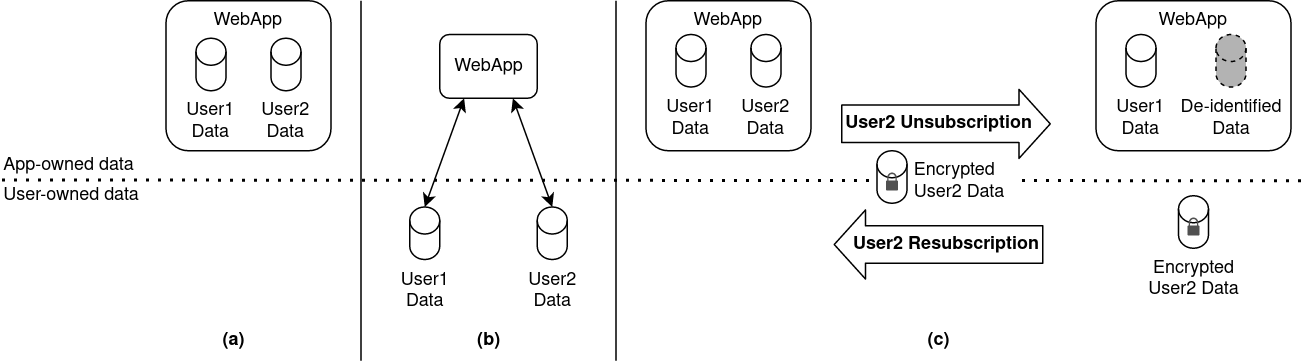
\includegraphics[width=\textwidth]{img/worlds}
%
%    \caption{\textbf{(a)} The current web application paradigm, in which applications maintain and
%    own user data; \textbf{(b)} A paradigm that decouples user data from web applications, giving users ownership of their data;
%    \textbf{(c)} \name, which allows users to switch between privacy-preserving unsubscribed mode (right) and identity-revealing subscribed mode (left).}
%    \label{fig:world}
%\end{figure*}
%
Web applications today own, store, and sell user data, often without the user's knowledge or
explicit consent~\cite{nytimes:fb, npr:data}. This both violates users' right for privacy, and has
dangerous consequences for both users and application developers as data leaks lead to loss of
livelihoods and lawsuits~\cite{breach:amazon,breach:twitter, breach:fb, breach:marriott,
breach:quora}.
%Granting web applications complete ownership of personal data clearly fails to
%protect users' privacy.

Although users want stronger privacy, completely decoupling user data from applications results in a
potentially even less desirable world. While possible~\cite{solid, amber, w5, blockstack, bstore}, such a
model hinders service-side computation and application performance, and requires users to manage
long-time security and storage of their data, leading to a lack of adoption in practice (Section~\ref{sec:related}).

This paper proposes \name, a new paradigm that grants users flexible privacy when using web
applications, balancing users' desire for privacy with their desire for application utility. In
\name, users subscribe to applications by granting a time-limited lease to their data, with the
provision that the application may retain only de-identified information once the user unsubscribes.
Users flexibly switch between a privacy-preserving unsubscribed mode and an identity-revealing
subscribed mode at any time without permanently losing their data. \name contrasts
with the current web application paradigm for data ownership, in which applications have complete
ownership, and the other extreme in which the user has complete data ownership.% (see Figure~\ref{fig:world}).

\name benefits users: they can choose privacy at any time, without
permanently losing their accounts or affecting the utility of the applications for others.  Just as
importantly, \name also benefits application developers. Recent laws such as the
European Union's General Data Protection Regulation (GDPR)~\cite{eu:gdpr} and California's Consumer
Privacy Act (CCPA)~\cite{ca:privacy-act} codify users' rights to data ownership, granting users the
right to request erasure of information related to them. Supporting \name enables
applications to comply with these legal mandates, while still allowing its departing users to easily
come back: if applications must let users leave, it is in their best interest to make it easy for
them to return.

Furthermore, applications can continue to operate using their current revenue model, maintaining
performance, reliability, and utility for their users.  Because applications retain use of
subscribed users' data, and de-identified data of unsubscribed users, applications optimize the
amount of data available to generate profit and provide utility for subscribed users. The
application holds only identifying data for subscribed users, reducing the amount of
compromising data in the system to only those users who have actively agreed to temporarily give up
their privacy.

Realizing \name poses a number of technical challenges.
Unsubscription and resubscription requires complex and fragile data transformations: developers must
selectively retain unsubscribed users' data for legal or application purposes while properly
de-identifying this data, a non-trivial task in the face of subtle inference attacks (\eg tags on a
user's post can identify the user). De-identification and data removal needs to be reversible,
allowing the user to resubscribe at any time to their last-known subscribed state.

To make \name a reality, we model application data as an abstract \emph{entity graph}, and
represent unsubscription and resubscription as transformations of this graph.
\emph{Ghost entities} allow transformations to achieve both data retention and de-identification,
and declarative \emph{ghost policies} specify reversible transformations upon unsubscription.
We design and implement \sys, a practical system that systematically automates this transformation for new and existing applications, helping developers realize the \name paradigm without onerous labor.
%that takes a developer-specified unsubscription policy for the application's entity
%graph, and ensures that
%that requires developers only to specify an abstract unsubscription policy on the
%helps developers of databased-backed web applications automatically achieve correct, privacy-compliant user unsubscription and
%resubscription without onerous labor.
\fi
